% CVPR 2022 Paper Template
% based on the CVPR template provided by Ming-Ming Cheng (https://github.com/MCG-NKU/CVPR_Template)
% modified and extended by Stefan Roth (stefan.roth@NOSPAMtu-darmstadt.de)

\documentclass[10pt,twocolumn,letterpaper]{article}

%%%%%%%%% PAPER TYPE  - PLEASE UPDATE FOR FINAL VERSION
% \usepackage[review]{cvpr}      % To produce the REVIEW version
% \usepackage{cvpr}              % To produce the CAMERA-READY version
\usepackage[pagenumbers]{cvpr} % To force page numbers, e.g. for an arXiv version

% Include other packages here, before hyperref.
\usepackage{graphicx}
\usepackage{amsmath}
\usepackage{notoccite}

\usepackage{amssymb}

\usepackage{booktabs}


% It is strongly recommended to use hyperref, especially for the review version.
% hyperref with option pagebackref eases the reviewers' job.
% Please disable hyperref *only* if you encounter grave issues, e.g. with the
% file validation for the camera-ready version.
%
% If you comment hyperref and then uncomment it, you should delete
% ReviewTempalte.aux before re-running LaTeX.
% (Or just hit 'q' on the first LaTeX run, let it finish, and you
%  should be clear).
\usepackage[pagebackref,breaklinks,colorlinks]{hyperref}


% Support for easy cross-referencing
\usepackage[capitalize]{cleveref}
\crefname{section}{Sec.}{Secs.}
\Crefname{section}{Section}{Sections}
\Crefname{table}{Table}{Tables}
\crefname{table}{Tab.}{Tabs.}


%%%%%%%%% PAPER ID  - PLEASE UPDATE
\def\cvprPaperID{56757} % * Enter the CVPR Paper ID here
\def\confName{CVPR}
\def\confYear{2024}




\begin{document}

%%%%%%%%% TITLE - PLEASE UPDATE
\title{A Report on Mainstream Image Recognition Technologies in Computer Vision }

\author{Liu Ziqi\\
2021300130\\
Northwestern Polytechnical University\\
{\tt\small 1114709266@qq.com}
% For a paper whose authors are all at the same institution,
% omit the following lines up until the closing ``}''.
% Additional authors and addresses can be added with ``\and'',
% just like the second author.
% To save space, use either the email address or home page, not both
% \and
% Second Author\\
% Institution2\\
% First line of institution2 address\\
% {\tt\small secondauthor@i2.org}
}
\maketitle

%%%%%%%%% ABSTRACT
\begin{abstract}
  The purpose of this paper is to present a report and review of fundamental concepts in the field of computer vision, including the application of traditional image descriptors (such as HoG, SIFT, etc.) in tasks such as image recognition, as well as the application of deep learning methods (CNN, RNN, Transformer, etc.) and transfer learning in computer vision tasks such as image recognition.
  %  Additionally, the paper will discuss the use of large-scale visual or multimodal models such as SAM, Dino, and GPT-4V.
\end{abstract}

%%%%%%%%% BODY TEXT
\section{Introduction}
\label{sec:intro}

The field of computer vision has experienced explosive development in recent years, transitioning from manual feature extraction methods for images to the automatic extraction of image features using deep learning techniques. This shift has led to significant improvements in model performance and has contributed to advancements in various domains. This report aims to introduce representative algorithms from different periods of computer vision development, providing a comprehensive understanding of the field's evolution and laying a solid foundation for future research.
% With the emergence of ChatGPT and the increase in computational power, large-scale models such as SAM, Dino, and GPT-4V have also come into focus. 
%-------------------------------------------------------------------------

%------------------------------------------------------------------------
\section{Method}
\label{sec:formatting}

This report will use image recognition tasks as an example to sequentially elucidate representative algorithms in the field of computer vision in chronological order.

Section 2.1 will include an introduction to traditional image descriptors, Section 2.2 will cover an overview of deep learning methods, Section 2.3 will focus on the application of transfer learning in image recognition, and Section 3.4 will introduce current large-scale visual or multimodal models.

%-------------------------------------------------------------------------
\subsection{Traditional Image Descriptors}

Firstly, an image descriptor is a simplified representation of an image, containing only the most important information about the image. By using image descriptors, we can obtain specific features of the image.

\subsubsection{SIFT}
   SIFT \cite{Alpher02} (Scale-invariant feature transform) is a classic feature point extraction and description algorithm in computer vision. This method was first published by David Lowe at the International Conference on Computer Vision (ICCV) in 1999 and was further refined and published in the International Journal of Computer Vision (IJCV) in 2004. SIFT features have several advantages:

1. They describe the local features of an image and maintain invariance to rotation (achieved by aligning the main orientation during feature descriptor generation), scale (ensured through the use of a difference of Gaussian pyramid), and brightness (ensured through feature normalization). They also exhibit robustness to changes in viewpoint, affine transformations, noise, and other variations.

2. They possess good uniqueness and rich information content, making them suitable for fast and accurate matching in large feature databases.

3. They exhibit multiplicity, meaning even a few objects can generate a large number of SIFT features.

4. When optimized, SIFT matching algorithms can achieve real-time performance.

5. They can easily be combined with other feature vectors.

The SIFT feature algorithm consists of four parts:

1) Scale-space extrema detection - Key point detection:
To search for potential interest points (key points) that should be present at different scales and levels of blur, the algorithm first computes the difference of Gaussian images.

First, the original image is blurred at different levels, increasing the variance to create a Gaussian scale space. Each image in this scale space undergoes a series of isotropic downsampling, resulting in a Gaussian scale pyramid representing different spatial scales.

Next, within the same Gaussian scale pyramid, the differences mainly arise from varying degrees of Gaussian blur. To detect feature points that exist under different blur conditions, the algorithm uses the difference of Gaussian (DoG) instead of the Laplacian of Gaussian (LoG) due to its simpler computation. The calculation method is as follows: 



\begin{align}
	D(x,y,\sigma)
	& = [G(x,y,k\sigma)-G(x,y,\sigma)]*I(x,y)\\
	& = L(x,y,k\sigma)-L(x,y,\sigma)
\end{align}
where $G(x,y,k\sigma)$ is the Gaussian function, and $L(x,y,\sigma)$ represents the Gaussian scale space of the image.

In other words, subtracting two images with different levels of Gaussian blur in the Gaussian space results in the response image of the difference of Gaussians. (Here, k represents the Gaussian variance of the two adjacent images multiplied by k). By subtracting each pair of adjacent images within the same group, the difference of Gaussian pyramid is obtained.

Next, in order to find the extremum points, within the same pyramid, each pixel needs to be compared with all its image neighbors (physically adjacent pixels) and scale neighbors (adjacent Gaussian scale space) to determine if it is greater than/less than all its neighbors. If so, the point is considered an extremum point. In the Figure.\ref{fig1}, all the green points are the "neighbors" of the point x.



2) Key Point Localization: For each candidate key point, the final determination of its suitability, position, and scale is crucial. In SIFT feature extraction, key points are identified as extremal points of the pixel values in the DoG image neighborhood (including both the Gaussian scale neighborhood and the image neighborhood), as the DoG represents the gradient due to the differencing of pixel values.However, the local extremal points in the DoG are obtained through discrete space search and may not necessarily be true extremal points. Therefore, it is necessary to eliminate points that do not meet the conditions. This can be achieved by curve fitting using the scale-space DoG function to find extremal points, essentially removing points with highly asymmetric local curvature in the DoG. This step primarily eliminates feature points with contrast below a certain threshold and unstable edge response points (achieved through detecting principal curvatures).

3) Orientation Assignment for Key Points: One or multiple orientations are assigned to each key point based on the image's gradient direction. After the previous steps, feature points that exist at different scales have been identified. In order to achieve rotation invariance, it is necessary to assign orientations to the feature points. For a particular feature point, its corresponding Gaussian scale image can be determined, and the gradient magnitude and orientation angles of the points within a 3x1.5 times the standard deviation range centered on this feature point can be computed:


\begin{figure}
  \centering % 居中显示图像
  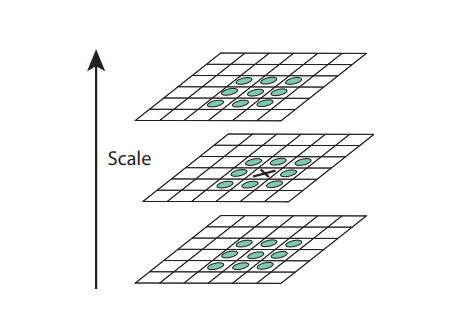
\includegraphics[width=0.5\textwidth]{image1.png} % 替换"image_file.png"为你自己的图像文件名及路径
  \caption{all the green points are the "neighbors" of the point x.} % 替换成你想要的图像标题或说明
  \label{fig1}
\end{figure}
	
  \begin{eqnarray}
		\theta(x,y)=arctan\frac{L(x,y+1)-L(x,y-1)}{L(x+1,y)-L(x-1,y)}
  \end{eqnarray}

The interval [0,360°] can be divided into 10 ranges, and the gradient histogram can be computed by accumulating the gradients within each range. The peak of the histogram represents the dominant orientation of the feature point (in practice, additional operations such as smoothing and interpolation should be applied).

In the gradient histogram, the presence of a bin value that accounts for 80\% of the total energy can indicate an auxiliary direction for the feature point. Consequently, a feature point may detect multiple directions (or, equivalently, produce multiple feature points with the same coordinates and scale but different orientations).
  
Lowe stated in his paper that 15\% of the keypoints have multiple orientations, and these points are crucial for the stability of matching.
  
Once the dominant orientation of the feature point is determined, each feature point can be characterized by three pieces of information (x, y, $\sigma$, $\theta$), representing its position, scale, and orientation. This information defines a SIFT feature region, which is represented by its center (indicating the feature point position), radius (indicating the scale of the keypoint), and an arrow (indicating the dominant orientation). Feature points with multiple orientations can be duplicated, and the orientation values can be assigned to the duplicated feature points, resulting in multiple feature points with the same coordinates and scale but different orientations.

4)Key point descriptors: the gradient, scale, and position are all determined. Then they are transformed into a representation that can effectively handle image distortion, lighting, and other conditions.

5)During the final detection, a database containing a large amount of trained image feature data will be used. The detection image will be compared with the feature data in the database, and recognition will occur when a sufficient number of matching features, at least three, are found.\cite{siftblog}


\subsubsection{HOG}

The HOG method\cite{Alpher03}, proposed in 2005, is now a popular feature descriptor technique in computer vision and image processing. It analyzes the distribution of edge directions within an object to describe its shape and appearance. The representation and shape of local targets can be well described by the density distribution of gradients or edge directions. The HOG method involves computing the gradient magnitude and direction for each pixel in the image, and then dividing the image into small cells. The original paper was aimed at effectively extracting pedestrian features. In Figure. \ref{fig2}

\begin{figure}
  \centering % 居中显示图像
  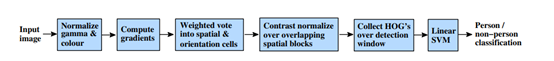
\includegraphics[width=0.5\textwidth]{image2.png} % 替换"image_file.png"为你自己的图像文件名及路径
  \caption{The process of the HOG algorithm in the original paper.} % 替换成你想要的图像标题或说明
  \label{fig2}
\end{figure}

The specific operation steps are as follows: first, normalize the image pixels to reduce the impact of lighting changes on the results when obtaining image features. Then, calculate the gradient and direction of the image in blocks, store them in histograms, concatenate the histograms of different blocks, and then normalize again to obtain the complete feature vector of the image. At this point, the image features have been obtained and can be further processed.\cite{exampleblog}
%-------------------------------------------------------------------------
\subsection{Deep Learning Method}

In recent years, with the improvement of computing power, deep learning methods have also achieved great success. Unlike traditional feature extraction, deep learning methods automatically learn the representation of data through neural networks, eliminating the need for manual design of feature extractors. Deep learning models can be trained end-to-end with a large amount of data, automatically learning the feature representation in the data, thereby better capturing complex patterns and features in the data. This has led to significant progress in many fields, especially in computer vision, natural language processing, and speech recognition. In summary, traditional methods require manual design of feature extractors, while deep learning methods learn the representation of data through neural networks. Representative examples include CNN\cite{Alpher04}, RNN\cite{Alpher05}, and the Transformer\cite{vaswani2017attention}, which has recently transitioned from the NLP field to the field of vision.

\subsubsection{CNN}

Convolutional Neural Network (CNN) is a type of deep learning model mainly used for processing and analyzing data with grid-like structures, such as images and videos. The design of CNN is inspired by the working principles of the human visual system, and it has achieved great success in the fields of image recognition, computer vision, and pattern recognition.

The basic structure of CNN includes convolutional layers, pooling layers, and fully connected layers. The convolutional layers extract features from the images through convolution operations, such as edges, textures, etc. The pooling layers are used to reduce the dimension of feature maps, decrease the number of parameters, while retaining important features. The fully connected layers are used to map the extracted features to different categories for the final classification or regression tasks.

The training of CNN is usually carried out through the backpropagation algorithm, using a large amount of labeled data for supervised learning. The emergence of CNN marks the formal rise and rapid development of deep learning algorithms. However, CNN also has certain limitations, such as a relatively large dependence on training samples, requiring a large amount of high-quality sample data support. In addition, the modeling effect for long-term dependencies is not ideal, resulting in more redundancy or poor processing effects when dealing with related entities. Therefore, in recent years, some variant CNN structures have also achieved great success, such as the introduction of residual blocks in residual networks, as well as the upcoming introduction of RNN, Transformer, and so on.



\subsubsection[short]{RNN}

RNN is a type of neural network, similar to deep neural network, and generative adversarial network, and so on. RNN is very effective for data with sequential characteristics, as it can explore the temporal and semantic information in the data. In comparison to CNN, which does not incorporate context in training the model and instead trains the label of a particular sample separately, RNN emerged. The basic architecture of the RNN network model is shown in Figure \ref{fig3}.
\begin{figure}
  \centering % 居中显示图像
  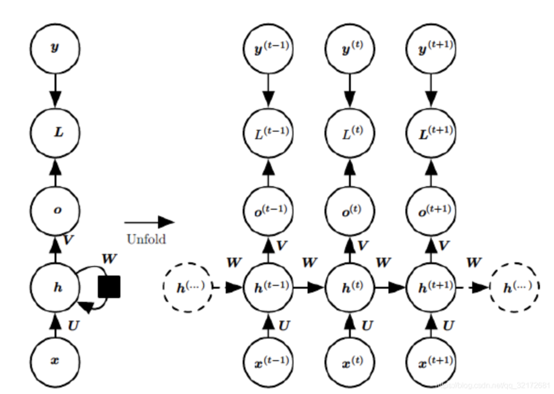
\includegraphics[width=0.5\textwidth]{image3.png} % 替换"image_file.png"为你自己的图像文件名及路径
  \caption{The basic architecture of the RNN network} % 替换成你想要的图像标题或说明
  \label{fig3}
\end{figure}


The key difference between recurrent neural networks (RNNs) and CNNs is that RNNs process current and previous inputs in a time-sequential manner, using their output as a combined input for the next iteration.
However, traditional RNNs have some limitations, including:

1. Long-term dependency problem: Traditional RNNs often encounter the issues of vanishing or exploding gradients when processing long sequential data, making it difficult to capture long-term dependency relationships.

2. Limited internal memory: Traditional RNNs have limited internal memory capacity, making it challenging to effectively capture important information in long sequences.

3. Difficulty in parallelization: Due to the temporal dependency of RNNs, it is difficult to effectively parallelize data processing, which affects the efficiency of training and inference.

4. Sensitivity to input sequence length: Traditional RNNs are sensitive to the length of input sequences, often leading to decreased performance when the input sequence is long.

To overcome the limitations of traditional RNNs, researchers have proposed a series of improved models, such as Long Short-Term Memory (LSTM), Gated Recurrent Unit (GRU), which have partially addressed some of the problems of traditional RNNs. In addition, there are also Attention-based models, such as Transformer, which have achieved great success in processing sequential data.

\subsubsection[short]{Transformer}

Transformer originated from the 2017 paper "Attention is all you need" by Google, initially used for machine translation with great success. Since then, the Transformer has excelled not only in the field of NLP but also demonstrated impressive performance in areas such as computer vision and recommendation systems. Particularly in 2020, it can be considered the prime time for the Transformer, as models based on it dominated various rankings in the field of computer vision. The following will introduce its principles and its applications in the field of computer vision.The basic architecture of the RNN network model is shown in Figure \ref{fig4}.

\begin{figure}
  \centering % 居中显示图像
  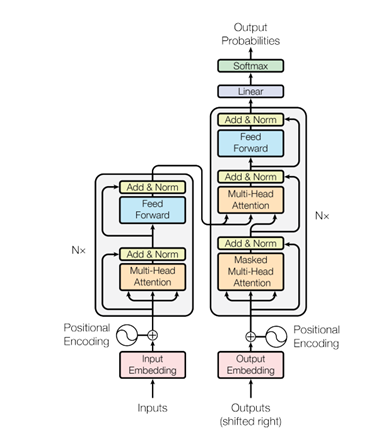
\includegraphics[width=0.5\textwidth]{image4.png} % 替换"image_file.png"为你自己的图像文件名及路径
  \caption{The basic architecture of the Transformer} % 替换成你想要的图像标题或说明
  \label{fig4}
\end{figure}

The Transformer consists mainly of an encoder, a decoder, and their connections. The encoder and decoder are responsible for transforming input and output into feature vectors, but the truly influential part of the transformer is its proposed Attention  shown in Figure \ref{fig5}.

\begin{figure}
  \centering % 居中显示图像
  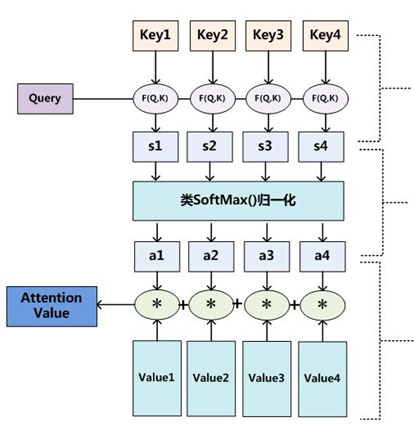
\includegraphics[width=0.5\textwidth]{image5.png} % 替换"image_file.png"为你自己的图像文件名及路径
  \caption{Basic principles of Attention.} % 替换成你想要的图像标题或说明
  \label{fig5}
\end{figure}

Stage 1: Calculate the similarity between Query and each Key to obtain a similarity score.

Stage 2: Convert the s scores into a probability distribution between [0,1] using softmax.

Stage 3: Use [a1, a2, a3...an] as the weight matrix to perform weighted summation on the Value to obtain the final Attention value.

\begin{eqnarray}
  A(Q,S)=\sum^{L_x}_{i=1}Sim(Q,Key_i)*V_i
\end{eqnarray}

In a typical Encoder-Decoder framework for tasks, the input Source and output Target content are different. For example, in English to Chinese machine translation, the Source is an English sentence, and the Target is the corresponding translated Chinese sentence. The Attention  occurs between the elements of the Target and all elements of the Source. On the other hand, Self-Attention, as the name suggests, refers to the Attention  not between the Target and Source, but within the elements of the Source or within the elements of the Target. It can also be understood as the Attention calculation  that occurs in the special case where Target equals Source.

\subsection{Transfer Learning}

Transfer Learning is a machine learning method that leverages existing knowledge to assist in solving new problems. It can effectively address challenges such as limited data and difficult labeling, enhancing the model's generalization ability. Typically, this is achieved through pre-trained models. Pre-training involves training a model on a large dataset and then fine-tuning it on a new task.
\begin{figure}
  \centering % 居中显示图像
  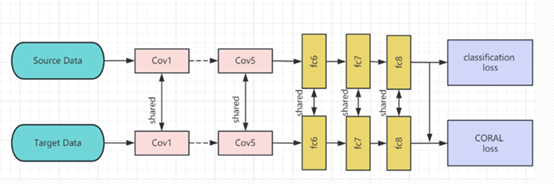
\includegraphics[width=0.5\textwidth]{image6.png} % 替换"image_file.png"为你自己的图像文件名及路径
  \caption{Basic principles of Deep Coral.} % 替换成你想要的图像标题或说明
  \label{fig6}
\end{figure}

In 2014, researchers introduced a neural network called DANN (Domain Adaptive Neural Network) at the Pacific Rim International Conference on Artificial Intelligence (PRICAI). DaNN falls under the category of Domain Adaptation. Domain adaptation is a crucial branch of transfer learning that aims to map data from different distributions in the source domain and target domain to the same feature space. The objective is to find a metric criterion to minimize the "distance" in this space. Once a classifier is trained on the labeled source domain data, it can be directly applied to classify target domain data. Mainstream methods include Deep Coral and DANN shown in Figure \ref{fig6} and Figure \ref{fig7}.




\section{Experiment}


\begin{figure}
  \centering % 居中显示图像
  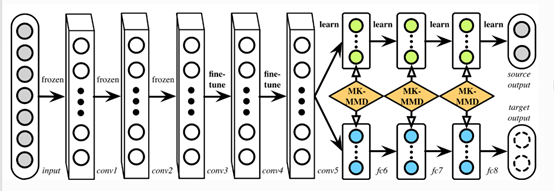
\includegraphics[width=0.5\textwidth]{image7.png} % 替换"image_file.png"为你自己的图像文件名及路径
  \caption{Basic principles of DANN.} % 替换成你想要的图像标题或说明
  \label{fig7}
\end{figure}

In this chapter, various computer vision algorithms mentioned above were employed to achieve several effects. The examples are listed below.

Traditional image descriptors are generally characterized by strong theoretical foundations. However, due to their widespread use, they are often encapsulated into well-established methods in the field of computer vision. These methods can be easily invoked when needed. The  image in Figure \ref{fig8} provides a visual example of utilizing the SIFT method for feature description in computer vision.

\begin{figure}
  \centering % 居中显示图像
  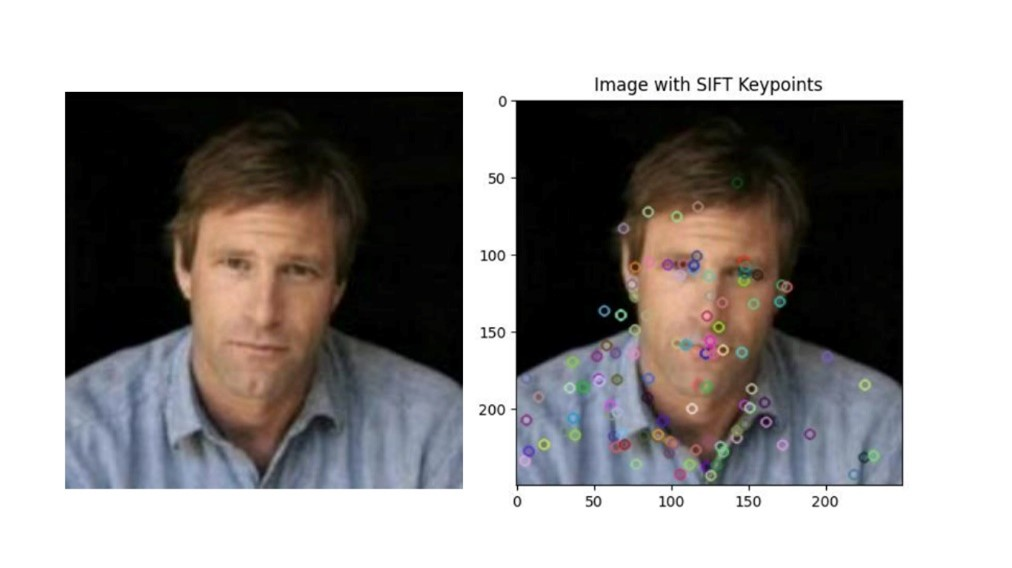
\includegraphics[width=0.5\textwidth]{image8.jpg} % 替换"image_file.png"为你自己的图像文件名及路径
  \caption{Each annotated circle in the image represents a feature point. These feature points are utilized during image classification to perform matching and selection.} % 替换成你想要的图像标题或说明
  \label{fig8}
\end{figure}

For the CNN experiment in this study, the performance of a Convolutional Neural Network (CNN) was evaluated using the VGG-16 architecture as a representative example. The evaluation was conducted on the CIFAR-10 dataset for image classification.


\begin{figure}
  \centering % 居中显示图像
  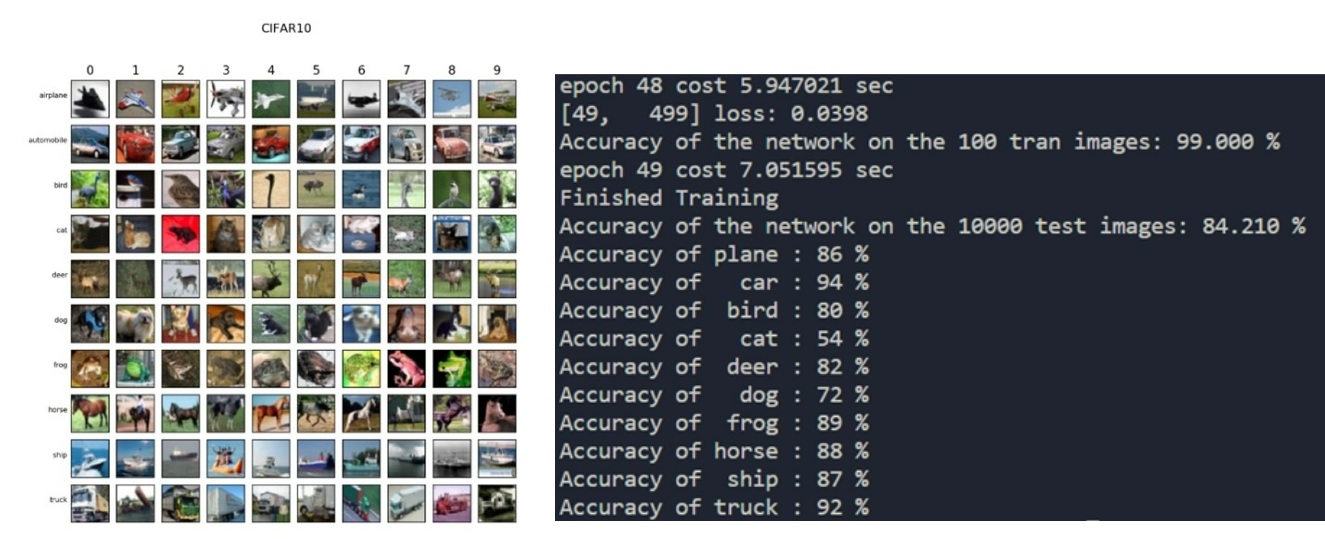
\includegraphics[width=0.5\textwidth]{image9.png} % 替换"image_file.png"为你自己的图像文件名及路径
  \caption{The left image shows a partial display of the CIFAR-10 dataset, while the right image illustrates the results of the training process.} % 替换成你想要的图像标题或说明
  \label{fig9}
\end{figure}

The CIFAR-10 dataset in Figure \ref{fig9} consists of 60,000 32x32 color images, distributed across 10 categories, with each category containing 6,000 images. Among these, 50,000 images are used for training, and 10,000 images are designated for testing. The dataset is divided into 5 training batches and 1 testing batch, each containing 10,000 images. The testing batch comprises 1,000 randomly selected images from each category.The training batches contain the remaining images, with some training batches potentially having more images for a particular category than others. Each training batch includes 5,000 images from various categories. The classes are mutually exclusive, meaning that an image from one category will not appear in any other category.
The image on the right side of Figure \ref{fig9} depicts the training process and results of this experiment.
\begin{figure}
  \centering % 居中显示图像
  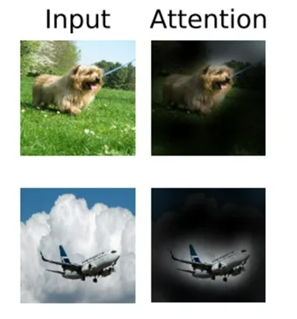
\includegraphics[width=0.5\textwidth]{image10.png} % 替换"image_file.png"为你自己的图像文件名及路径
  \caption{The visualization of Attention.} % 替换成你想要的图像标题或说明
  \label{fig10}
\end{figure}

In the field of computer vision, CNNs have dominated, while in natural language processing (NLP), Transformers have become standard. In recent years, there has been a significant number of articles on the cross-application of Transformers to computer vision. Most of these approaches are based on two main ideas:

(1) Combining attention mechanisms with CNNs.

(2) Replacing certain CNN structures with attention mechanisms while keeping the overall architecture unchanged.

Figure \ref{fig10} visualizes the Attention method, providing an explanation of the attention mechanism's capability to handle contextual relationships and capture essential information.

Due to limitations in the experimental environment, this implementation\cite{dosovitskiy2020image} may not be replicated independently. However, Figure \ref{fig11} showcases the experimental results obtained by the authors of this paper.

\begin{figure}
  \centering % 居中显示图像
  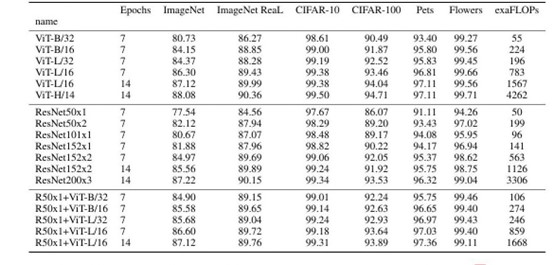
\includegraphics[width=0.5\textwidth]{image11.jpg} % 替换"image_file.png"为你自己的图像文件名及路径
  \caption{The testing results of the Transformer on different datasets and its comparison with other methods.} % 替换成你想要的图像标题或说明
  \label{fig11}
\end{figure}

On the experimental level, it was observed that ViT\cite{dosovitskiy2020image} (Vision Transformer) has a performance upper limit higher than ResNet. In other words, under conditions of a sufficiently large dataset, Attention s can fully replace CNNs (Convolutional Neural Networks).

\begin{figure}
  \centering % 居中显示图像
  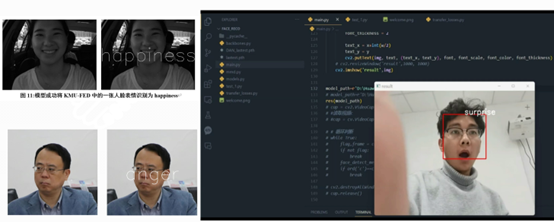
\includegraphics[width=0.5\textwidth]{image12.png} % 替换"image_file.png"为你自己的图像文件名及路径
  \caption{The figure represents experimental results on image recognition using transfer learning, specifically for facial expression recognition.} % 替换成你想要的图像标题或说明
  \label{fig12}
\end{figure}



The training for transfer learning was conducted locally, shown as Figure \ref{fig12} and Table \ref{tab1}, and the experiment utilized two transfer learning algorithms: DANN\cite{ganin2016domain} (Domain Adversarial Neural Network) and Deep Coral\cite{sun2016deep}. These algorithms were employed for image recognition, and the differences in experimental results were analyzed.

\begin{table}
  \centering
  \begin{tabular}{@{ } lc@ { }   lc@ { } }
    \toprule
    Method & Loss &   Acc(\%) \\
    \midrule
    DANN & 0.78 &   63.99\\
    DeepCoral & 0.69 &   62.56\\
    
    \bottomrule
  \end{tabular}
  \caption{The result of transfer learning method. }
  \label{tab1}
\end{table}

The experimental results indicate that the performance of both heterogeneous transfer learning approaches meets the basic requirements for discerning facial expressions. However, the accuracy of the training results is not overly precise. The possible reasons for this could be attributed to the following four points:

1. Significant Discrepancy Between Source and Target Domains:
   The images in the source domain, MMA FACIAL EXPRESSION, consist of European and American portraits, while the target domain comprises images of Asians. Due to the substantial facial differences between Europeans/Americans and Asians, this results in a lower accuracy.

2. Insufficient Training Iterations, Incomplete Model Fitting:
   Limited by training time and resources, we conducted training for 50 iterations. It is reasonable to believe that the lower test results may be due to incomplete model fitting resulting from the limited training iterations.

3. Improper Parameter Adjustment:
   Parameters of the transfer learning model may require more detailed adjustments and optimization to adapt to the target domain's data. In our case, we directly used default optimal parameters from other transfer learning tasks as hyperparameters for this task. This improper parameter setting may have contributed to the suboptimal results.

   For the two algorithms implemented in this task, the accuracy of DANN is superior to Deepcoral. This further proves that directly performing feature transformation and re-fitting on the data source and target domain is more effective than simply reducing cross-domain losses. It also provides valuable insights for our future algorithm design considerations.

%------------------------------------------------------------------------
\section{Conclusion}

This paper aims to present a report and review of fundamental concepts in the field of computer vision. It includes the application of traditional image descriptors such as HoG, SIFT, etc., in tasks like image recognition. Additionally, the paper explores the application of deep learning methods, including CNN, RNN, Transformer, etc., as well as transfer learning in computer vision tasks such as image recognition. The paper emphasizes the importance of both traditional and deep learning approaches in the field of image recognition. Traditional methods like HoG and SIFT are utilized for image description, while deep learning methods like CNN, RNN, and Transformer demonstrate strong performance in computer vision tasks. Furthermore, the paper focuses on the application of transfer learning in computer vision, highlighting its potential to enhance model performance and generalization. Overall, the paper provides readers with a comprehensive understanding of key concepts in the field of computer vision and discusses the advantages and limitations of different approaches in addressing image recognition challenges.

The experimental code for the paper has been uploaded to GitHub. For detailed information, please visit the website:
\url{https://github.com/Michael8023/cv_report}.



%%%%%%%%% REFERENCES
{\small
\bibliographystyle{unsrt}
% \bibliographystyle{ieee_fullname}
\bibliography{egbib}
}

\end{document}
